% ════════════════════════════════════════════════════════════════
\section{Wykład 8}
\subsection{Dowód optymalności algorytmu Huffmana}
% ════════════════════════════════════════════════════════════════

Kody prefiksowe $\iff$ regularne drzewa binarne.

$C$ -- alfabet, $f: C \to \N$ funkcja częstości, $d_T(c)$ -- głębokość liścia reprezentującego $c$ w drzewie $T$ reprezentującym kod prefiksowy.

\begin{flalign*}
	B(T) = \sum_{c\in C} f(c) \cdot d_T(c) \longleftarrow \min && &&
\end{flalign*}

\begin{lemma} \label{lemma:huffman:1}
	{Lemat 1}
	Niech $x$ i $y$ będą najrzadziej występującymi znakami z $C$. Istnieje optymalny kod prefiksowy, w którym słowa kodowe $x$ i $y$ mają tę samą długość i różnią się tylko na ostatnim bicie.
\end{lemma}

\begin{proof}
	Znajdziemy drzewo reprezentujące optymalny kod prefiksowy, w którym liście reprezentujące $x$ i $y$ mają wspólnego rodzica i mają największą głębokość w drzewie.
	
	Niech $T$ będzie dowolnym drzewem reprezentującym optymalny kod prefiksowy i niech $a$ i $b$ będą dwoma liśćmi o tym samym rodzicu i najmniejszej głębokości w $T$.
	Bez straty ogólności możemy przyjąć, że $f(x) \leq f(y)$ i $f(a) \leq f(b)$.
	$f(x)$ i $f(y)$ są najmniejszymi kluczami, więc $f(x) \leq f(a)$ i $f(y) \leq f(b)$.
	
	Niech $T'$ będzie drzewem powstałym z $T$ przez zamianę liści $x$ i $a$.
	\begin{flalign*}
		B(T) - B(T') &= \sum_{c \in C} f(c) \cdot d_T(c) - \sum_{c \in C} f(c) \cdot d_{T'}(c) = f(a) \cdot d_T(a) + f(x) \cdot d_T(x) - f(a) \cdot d_{T'}(a) - f(x) \cdot d_{T'}(x) = && \\
		&= f(a) \cdot d_T(a) + f(x) \cdot d_T(x) - f(a) \cdot d_T(x) - f(x) \cdot d_T(a) = f(a) (d_T(a) - d_T(x)) - f(x) (d_T(a) - d_T(x)) = && \\
		&= \underbrace{(f(a) - f(x))}_{\geq 0} \underbrace{(d_T(a) - d_T(x))}_{\geq 0} \geq 0 &&
	\end{flalign*}
	
	Zatem $B(T) \geq B(T')$, ale $B(T)$ najmniejsze możliwe, więc $B(T') = B(T)$ czyli $T'$ też reprezentuje optymalny kod prefiksowy. Analogicznie zamieniamy miejscami liście $y$ i $b$ i otrzymujemy drzewo $T''$ reprezentujące optymalny kod prefiksowy, które ma żądane własności.
\end{proof}

Z lematu~\ref{lemma:huffman:1} wynika, że można zacząć konstrukcję optymalnego drzewa połączeniem dwóch symboli o najmniejszej częstości.
\textbf{Zachłanny wybór} -- w każdym kroku algorytm łączy dwa wierzchołki o najmniejszych kluczach.

\begin{lemma} \label{lemma:huffman:2}
	{Lemat 2}
	Niech $A$ będzie alfabetem, a $f: A \to \N$ funkcją częstości. Niech $x$ i $y$ będą dwoma najrzadziej występującymi znakami w $A$. Niech $A' = (A \setminus \{x, y\}) \cup \{z\}$, gdzie $z \notin A$ i $f': A' \to \N$ będzie funkcją częstości taką, że dla każdego $c \in A' \setminus \{z\}$, $f'(c) = f(c)$ oraz $f'(z) = f(x) + f(y)$. Niech $T'$ będzie drzewem reprezentującym optymalny kod dla $(A', f')$. Niech $T$ będzie drzewem powstałym z $T'$ poprzez zastąpienie liścia $z$ wierzchołkiem wewnętrznym z dziećmi $x$ i $y$. $T$ reprezentuje optymalny kod prefiksowy dla $(A, f)$.
\end{lemma}

\begin{proof}
	Dla $c \in A \setminus \{x, y\}$, $d_T(c) = d_{T'}(c)$ a $d_T(x) = d_T(y) = d_{T'}(z) + 1$.
	Zatem:
	\begin{flalign*}
		B(T) &= \sum_{c \in A} f(c) \cdot d_T(c) = \sum_{c \in A \setminus \{x, y\}} f(c) \cdot d_T(c) + f(x) \cdot d_T(x) + f(y) \cdot d_T(y) = && \\
		&= \sum_{c \in A \setminus \{x, y\}} f'(c) \cdot d_{T'}(c) + f(x) (d_{T'}(z) + 1) + f(y) (d_{T'}(z) + 1) = && \\
		&= \sum_{c \in A \setminus \{x, y\}} f'(c) \cdot d_{T'}(c) + d_{T'}(z) (f(x) + f(y)) + f(x) + f(y) = \sum_{c \in A' \setminus \{z\}} f'(c) \cdot d_{T'}(c) + d_{T'}(z) \cdot f'(z) + f(x) + f(y) = && \\
		&= \sum_{c \in A'} f'(c) \cdot d_{T'}(c) + f(x) + f(y) = B(T') + f(x) + f(y) &&
	\end{flalign*}
	Stąd $B(T') = B(T) - f(x) - f(y)$.
	
	Przypuśćmy, że $T$ nie reprezentuje optymalnego kodu dla $(A, f)$. Niech $T''$ będzie drzewem reprezentującym kod prefiksowy dla $(A, f)$ takim, że $B(T'') < B(T)$. Z lematu~\ref{lemma:huffman:1} możemy wybrać $T''$ tak, aby $x$ i $y$ miały wspólnego rodzica i największą głębokość w $T''$. Niech $T'''$ będzie drzewem powstałym z $T''$ poprzez usunięcie liści $x$ i $y$, nadanie ich rodzicowi etykiety $z$ z kluczem $f(x) + f(y)$.
	$T'''$ reprezentuje kod prefiksowy dla $(A', f')$.
	
	Takim samym obliczeniem jak wcześniej (zamieniając wszystkie $T$ na $T''$, $T'$ na $T'''$) pokazujemy, że $B(T''') = B(T'') - f(x) - f(y)$.
	Mamy:
	\begin{flalign*}
		B(T''') = B(T'') - f(x) - f(y) < B(T) - f(x) - f(y) = B(T') && &&
	\end{flalign*}
	Sprzeczność z optymalnością $T'$ dla $(A', f')$.
	Zatem $T$ reprezentuje optymalny kod dla $(A, f)$.
\end{proof}

\begin{theorem}
	Algorytm Huffmana konstruuje drzewo reprezentujące optymalny kod prefiksowy.
\end{theorem}

\begin{proof}
	Indukcja po $n = \text{liczba symboli w alfabecie } C$.
	Dla $n=1, 2$ teza jest oczywista $\checkmark$.
	Niech $n > 2$.
	
	Po pierwszej operacji połączenia dostajemy alfabet $C' = (C \setminus \{x, y\}) \cup \{z\}$ i funkcję $f': C' \to \N$ taką, że $f'(c) = f(c)$ dla wszystkich $c \in C' \setminus \{z\}$ i $f'(z) = f(x) + f(y)$, gdzie $x$ i $y$ są znakami z $C$ o najmniejszych kluczach.
	Mamy $|C'| = n - 1$. Z założenia indukcyjnego algorytm znajduje drzewo $T'$ reprezentujące optymalny kod prefiksowy dla $(C', f')$. Na mocy lematu~\ref{lemma:huffman:2}, zastąpienie liścia $z$ w $T'$ wierzchołkiem z dziećmi $x$ i $y$ (co właśnie robi algorytm Huffmana) daje drzewo $T$ będące optymalnym kodem prefiksowym dla $(C, f)$.
\end{proof}

% ════════════════════════════════════════════════════════════════
\subsection{Szeregowanie zadań}
% ════════════════════════════════════════════════════════════════

Jak uszeregować zadania tak, aby średni czas ukończenia był jak najmniejszy?

\begin{example}{Szeregowanie zadań -- jeden procesor}
\begin{table}[H]
	\centering
	\renewcommand{\arraystretch}{1.2}
	\begin{NiceTabular}{c|c|c}[margin,hvlines]
		$i$ & zadanie & $t_i$ \\
		\hline
		1 & $z_1$ & 15 \\
		2 & $z_2$ & 8 \\
		3 & $z_3$ & 3 \\
		4 & $z_4$ & 10
	\end{NiceTabular}
\end{table}

Rozważmy uszeregowanie $z_1, z_2, z_3, z_4$:
\begin{flalign*}
	\frac{15 + (15+8) + (15+8+3) + (15+8+3+10)}{4} = \frac{15 + 23 + 26 + 36}{4} = \frac{100}{4} = 25 && &&
\end{flalign*}

Rozważmy uszeregowanie $z_3, z_2, z_4, z_1$:
\begin{flalign*}
	\frac{3 + (3+8) + (3+8+10) + (3+8+10+15)}{4} = \frac{3 + 11 + 21 + 36}{4} = 17 \frac{3}{4} && &&
\end{flalign*}

\textbf{Rozwiązanie:} Uszereguj zadania od najkrótszego do najdłuższego.
\end{example}

\paragraph{Problem 2}
Mamy 3 procesory. Pytanie jak poprzednio.

\begin{example}{Szeregowanie zadań -- trzy procesory}
\begin{table}[H]
	\centering
	\renewcommand{\arraystretch}{1.2}
	\begin{NiceTabular}{c|c|c|c|c|c|c|c|c|c}[margin,hvlines]
		Zadanie & $z_1$ & $z_2$ & $z_3$ & $z_4$ & $z_5$ & $z_6$ & $z_7$ & $z_8$ & $z_9$ \\
		\hline
		$t_i$ & 3 & 5 & 6 & 10 & 11 & 14 & 15 & 18 & 20
	\end{NiceTabular}
\end{table}

\textbf{Rozwiązanie:} Przydzielaj zadania do pierwszego wolnego procesora w kolejności od najkrótszego do najdłuższego.

\begin{figure}[H]
	\centering
	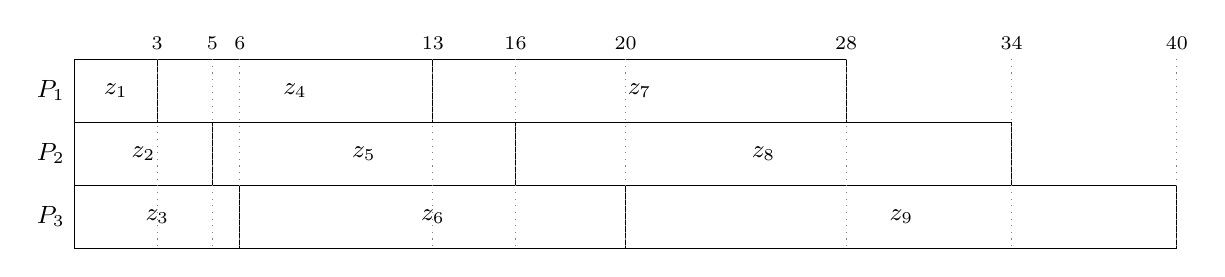
\begin{tikzpicture}[x=0.35cm, y=0.8cm, font=\small]
		% P1
		\draw (0, 2) rectangle (3, 3) node[midway] {$z_1$};
		\draw (3, 2) rectangle (13, 3) node[midway] {$z_4$};
		\draw (13, 2) rectangle (28, 3) node[midway] {$z_7$};

		% P2
		\draw (0, 1) rectangle (5, 2) node[midway] {$z_2$};
		\draw (5, 1) rectangle (16, 2) node[midway] {$z_5$};
		\draw (16, 1) rectangle (34, 2) node[midway] {$z_8$};

		% P3
		\draw (0, 0) rectangle (6, 1) node[midway] {$z_3$};
		\draw (6, 0) rectangle (20, 1) node[midway] {$z_6$};
		\draw (20, 0) rectangle (40, 1) node[midway] {$z_9$};

		\node[left] at (0, 2.5) {$P_1$};
		\node[left] at (0, 1.5) {$P_2$};
		\node[left] at (0, 0.5) {$P_3$};

		\foreach \x in {3, 5, 6, 13, 16, 20, 28, 34, 40} {
			\node[above, font=\scriptsize] at (\x, 3) {\x};
			\draw[gray, dotted] (\x, 3) -- (\x, 0);
		}
	\end{tikzpicture}
\end{figure}
\end{example}

W \textbf{Problemie 1} dla uszeregowania $z_{i_1}, z_{i_2}, \dots, z_{i_n}$ suma zakończeń zadań wynosi:
\begin{flalign*}
	\sum_{j=1}^n \sum_{k=1}^j t_{i_k} &= t_{i_1} + (t_{i_1} + t_{i_2}) + (t_{i_1} + t_{i_2} + t_{i_3}) + \dots + (t_{i_1} + \dots + t_{i_n}) = && \\
	&= n \cdot t_{i_1} + (n - 1) t_{i_2} + (n - 2) t_{i_3} + \dots + 1 \cdot t_{i_n} = \sum_{j=1}^n (n + 1 - j) t_{i_j} &&
\end{flalign*}

W \textbf{Problemie 2} (dla $3 \mid n$) dla uszeregowania $z_{i_1}, z_{i_2}, \dots, z_{i_n}$ suma czasów zakończeń wynosi:
\begin{flalign*}
	&t_{i_1} + t_{i_2} + t_{i_3} + (t_{i_1} + t_{i_4}) + (t_{i_2} + t_{i_5}) + (t_{i_3} + t_{i_6}) + (t_{i_1} + t_{i_4} + t_{i_7}) + (t_{i_2} + t_{i_5} + t_{i_8}) + (t_{i_3} + t_{i_6} + t_{i_9}) + && \\
	&+ \dots + (t_{i_1} + t_{i_4} + \dots + t_{i_{n-2}}) + (t_{i_2} + t_{i_5} + \dots + t_{i_{n-1}}) + (t_{i_3} + t_{i_6} + \dots + t_{i_n}) = && \\
	&= \frac{n}{3} (t_{i_1} + t_{i_2} + t_{i_3}) + \left(\frac{n}{3} - 1\right) (t_{i_4} + t_{i_5} + t_{i_6}) + \left(\frac{n}{3} - 2\right) (t_{i_7} + t_{i_8} + t_{i_9}) + \dots + 1 \cdot (t_{i_{n-2}} + t_{i_{n-1}} + t_{i_n}) = && \\
	&= \sum_{j=1}^n \left( \frac{n}{3} - \left\lfloor \frac{j-1}{3} \right\rfloor \right) t_{i_j} = \sum_{j=1}^n \left\lceil \frac{n+1-j}{3} \right\rceil \cdot t_{i_j} &&
\end{flalign*}

\begin{lemma}
	Niech $A_1 \geq A_2 \geq \dots \geq A_n$. Dla dowolnej permutacji $\Pi = (i_1, \dots, i_n)$ zbioru $[n]$ niech $f(\Pi) = \sum_{j=1}^n A_j \cdot t_{i_j}$. $f(\Pi)$ jest najmniejsze dla dowolnej permutacji $\Pi = (i_1, \dots, i_n)$ takiej, że $t_{i_1} \leq t_{i_2} \leq \dots \leq t_{i_n}$.
\end{lemma}

\begin{proof}
	Niech $\Pi = (i_1, \dots, i_n)$ będzie permutacją minimalizującą $f$. Przypuśćmy, że dla pewnych $k, l \in [n]$, $k < l$ ale $t_{i_k} > t_{i_l}$. Niech $\Pi' = (i'_1, i'_2, \dots, i'_n)$ będzie permutacją powstałą z $\Pi$ poprzez zamianę $i_k$ z $i_l$, tzn. $i'_j = i_j$ dla $j \in [n] \setminus \{k, l\}$, $i'_k = i_l$, $i'_l = i_k$. Wtedy:
	\begin{flalign*}
		f(\Pi) - f(\Pi') &= \sum_{j=1}^n A_j \cdot t_{i_j} - \sum_{j=1}^n A_j \cdot t_{i'_j} = A_k \cdot t_{i_k} + A_l \cdot t_{i_l} - A_k \cdot t_{i'_k} - A_l \cdot t_{i'_l} = && \\
		&= A_k \cdot t_{i_k} + A_l \cdot t_{i_l} - A_k \cdot t_{i_l} - A_l \cdot t_{i_k} = A_k(t_{i_k} - t_{i_l}) - A_l(t_{i_k} - t_{i_l}) = && \\
		&= \underbrace{(t_{i_k} - t_{i_l})}_{> 0} \cdot \underbrace{(A_k - A_l)}_{\geq 0} \geq 0 &&
	\end{flalign*}
	Zatem $f(\Pi') \leq f(\Pi)$, ale $\Pi$ minimalizuje $f$, więc $f(\Pi') = f(\Pi)$ i $\Pi'$ też minimalizuje $f$.
	Po pewnej liczbie takich zamian otrzymujemy permutację $\Pi_0 = (j_1, \dots, j_n)$ minimalizującą $f$ taką, że $t_{j_1} \leq t_{j_2} \leq \dots \leq t_{j_n}$.
\end{proof}

\textbf{Wniosek:} Nasze algorytmy szeregowania zadań są poprawne.
